\chapter{Background}
\label{sec:background}
In this section, the main algorithm used for this project will be mentioned as well as preliminaries regarding to computer vision.
\section{Computer Vision Preliminaries}
\label{sec:cvpre}
Before I go in to the details, let me introduce some necessary fundamentals.
\subsection{Image Format}
\label{sec:imageformat}
As far as this report is concerned, both RGB and depth images are used. RGB images have three channels, namely red, green and blue. Each of which has a value ranges from 0 to 255 which represents the respective intensity. The combination of the three channels will represent a pixel in a digital image. Unlike RGB, Grayscale (also know as black and white) images have only one channel and only possess the intensity information of a pixel. \cite{gray} 

The conversion from RGB to grayscale by the Luminosity method is :
\begin{equation}
 Grayscale = 0.21\times Red + 0.72\times Green + 0.07\times Blue
\end{equation}

Examples of a RGB image and it's corresponding Grayscale are shown in Figures \ref{fig:rgb} and \ref{fig:gray}

\begin{figure}
	\centering
	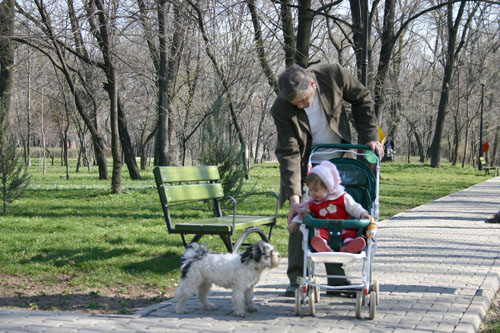
\includegraphics[width=0.8\linewidth]{Channel_digital_image_RGB_color.jpg}
	\caption[rgb image]{\label{fig:rgb}}  \textbf{RGB} 
\end{figure}

\begin{figure}
	\centering
	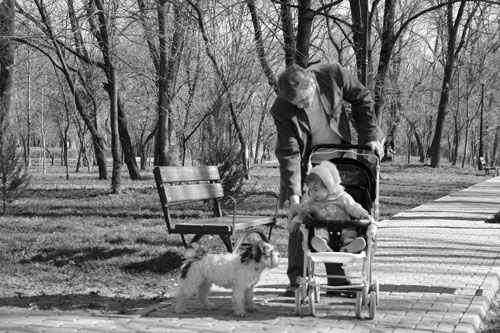
\includegraphics[width=0.8\linewidth]{Channel_digital_image_red.jpg}
	\caption[gray image]{\label{fig:gray}}  \textbf{Gray} 
\end{figure}

In addition to 2D images, due to the rise of depth sensor such as Microsoft Kinect. Depth images become available. Each pixel of a depth image contains the information of the distance from an object in a 3D scene to the viewpoint. An example of a depth image with its colour version is shown in Figure \ref{fig:depth}.

\begin{figure}
	\centering
	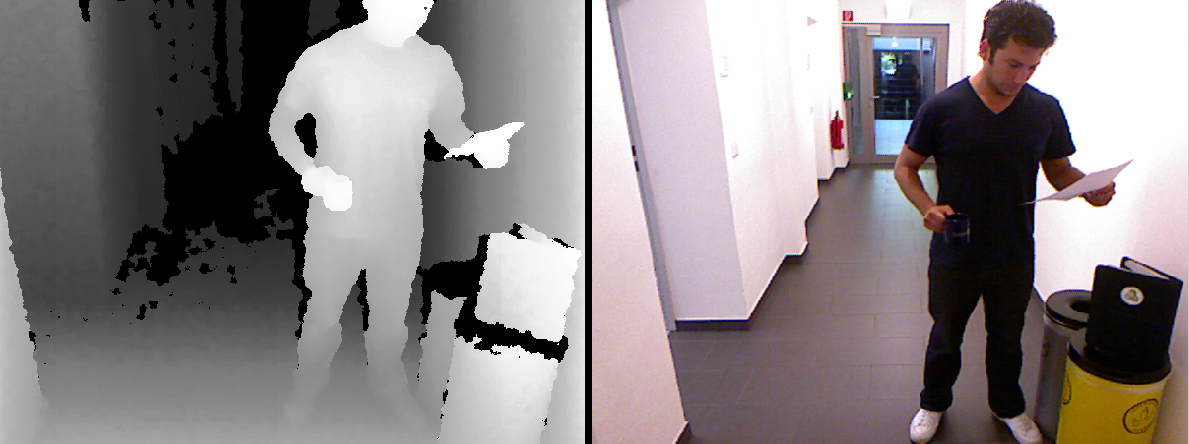
\includegraphics[width=0.8\linewidth]{depthandcolor.png}
	\caption[depth and colour images]{\label{fig:depth}}  \textbf{Depth and Colour} 
\end{figure}

\subsection{Euler Angles}
\label{sec:eulerangles}
Euler Angles are the most commonly used rotational coordinates. As far as this project is concerned, Euler angles are used to classify the head rotations. As shown in Fig \ref{fig:eulerangles}

\begin{figure}
	\centering
	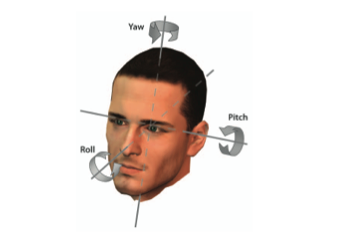
\includegraphics[width=0.8\linewidth]{headpose1.png}
	\caption[Euler Angles]{\label{fig:eulerangles}}  \textbf{The three degrees of freedom of a human head can be described by the egocentric rotation angles pitch, roll, and yaw \cite{HPS}} 
\end{figure}


%\section{Face Image analysis applications}
%\label{sec:faceapp}


%\section{General Object Detection Methods}
%\label{sec:objectD}

\section{Haar-Like Features}
\label{sec:HLfeatures}
The use of Haar-Like feature (as shown in Fig \ref{fig:hlfeature}) plays a big role in the scene of object detection. As mentioned in \cite{facedetect}, feature based systems perform better than pixel base systems. It is also known as rectangular features. In this project, only two rectangle feature is used which computes the difference between the sum of the pixels of two rectangular regions. One may notice, as the size of the rectangular region grows, the computation time will increase dramatically. Integral image is introduced to overcome this problem. \cite{facedetect}

\begin{figure}
	\centering
	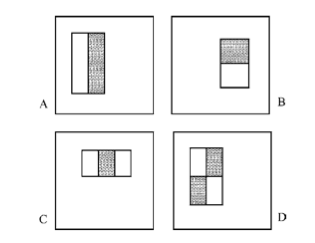
\includegraphics[width=0.8\linewidth]{hlfeature.png}
	\caption[Haar like Feature]{\label{fig:hlfeature}}  \textbf{A, B show the two rectangular feature whereas C and D show three rectangular feature and four rectangular feature respectively. The sum of the pixel values in the white rectangle is subtracted from the sum of the pixel values in the grey one. } \cite{facedetect}
\end{figure}

\subsection{Integral Image}
\label{sec:integralimage}
Feature computation is an important and necessary step in face image analysis but it could also be very time consuming as the size of the rectangular regions increase. As a result, integral image is used which enables fast computation. An integral image at location x, y contains the sum of the pixels above and to the left of x and y.(See Fig \ref{fig:integral1} \cite{integralimage} Analytically : 
\begin{equation}
sum(x,y)= \sum\limits_{a\leq x,b\leq y}i(a,b)
\end{equation}
Where $sum(x,y)$ is the pixel value at position (x,y) of the integral image and $i(a,b)$ is the pixel value at position (a,b) of the original image. Once integral images are created, sum within any rectangle can be computed by only referencing four points in the integral image. As shown in Fig \ref{fig:integral2}.

\begin{figure}
	\centering
	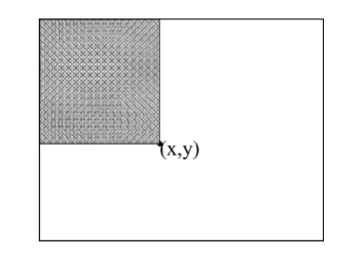
\includegraphics[width=0.8\linewidth]{integral1.png}
	\caption[Integral image]{\label{fig:integral1}}  \textbf{The value of the integral image at point(x,y) is the sum of all the pixels above and to the left  } \cite{integralimage}
\end{figure}

\begin{figure}
	\centering
	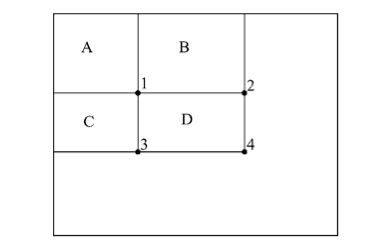
\includegraphics[width=0.8\linewidth]{integral2.png}
	\caption[Integral image referencing]{\label{fig:integral2}}  \textbf{If we are required to computer the sum of all the pixel values in D, the only 4 points we need to know is 1,2,3,4 since the value at 1 is A, the value at 2 is A + B, the value at 3 is A + C and the value at 4 is A + B + C + D, with a bit of algebra, it is not difficult to see that D = 4 + 1 - 2 - 3. }\cite{integralimage} 
\end{figure}



\section{Random Forest Framework}
\label{sec:RF}
In this section, Random Forest will be mentioned in detail since it is the algorithm used for this project. Random forest is first mentioned by Breiman in 2001 \cite{RFML}. And it had been widely used and explored in many applications since then. Before we discuss how to create a forest, let's look at how to build a decision tree first.
\subsection{Decision Trees fundamentals}
\label{subsec:Dtree}
"A tree is a set of nodes and edges organized in a hierarchical fashion" as can be seen in figure \ref{fig:decisiontree} \cite{DFMS,2dGFRF}. This structure is faster when it comes to searching the data space.  In contrast to graphs, loops does not exist in trees. In this project, only binary trees are considered. Intuitively, a decision is a tree which can make decision about the incoming data and it is built  in order to decompose complex problems into smaller pieces which are easier to solve. For example, we are given an image and asked to tell whether there is a snake inside that image. The constructed tree from the prior data set (different images with and without presence of snakes) will tell us the probability of a snake being in the image with the image given. And depending on the size of the training set and the parameters applied to build the decision trees, the results might be different. In a decision tree, leaf nodes contain either the probability distribution of the which class the incoming data belongs to (classification) or the value the incoming data should approximately take(regression) and non-leaf nodes contains stores binary tests which are applied to incoming data. To perform a test on unseen data, data is passed from the root of the tree and follows the test at each intermediate node until the leaf node is reached \cite{MVDT,DTBBR,IIDT}.

\begin{figure}
	\centering
	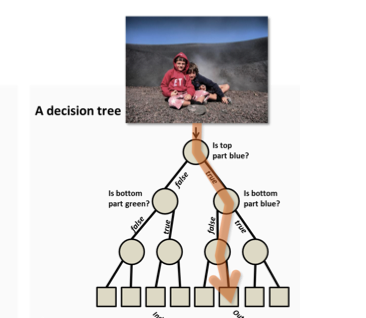
\includegraphics[width=0.6\linewidth]{decisiontree.png}
	\caption[decision tree]{\label{fig:decisiontree}} A decision tree that determines if the picture is taken outdoor or indoor. \cite{DFMS} 
\end{figure}

\subsection{Tree training}
\label{subsec:TTraining}

\begin{figure}
	\centering
	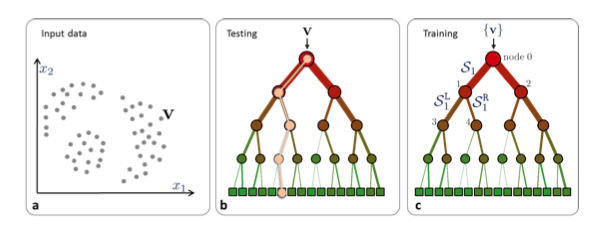
\includegraphics[width=0.6\linewidth]{treeTestTrain.png}
	\caption[Decision tree for 2D data]{\label{fig:treetesttrain}} Decision tree for 2D data clustering\cite{DFMS} 
\end{figure}

Building a tree is a supervised learning problem which requires the training data to be annotated with labels on the target value. For example, input data is in the form of $ \{ (\mathbf{x}_{i},y_{i})\}$, where $\mathbf{x}$ is in 2$\mathbf{D}$ space, $i$ is data label from 1 to $N$ and $y$ is the target value for $\mathbf{x}$.We want to construct the tree which can give the best representation for the associated data. Every data point is sent to the root node and the split function is chosen so that the information gain (discussed later in section \ref{subsec:EIG}) of that split is maximized.(as shown in Figure \ref{fig:treetesttrain} )This process is repeated after each split with the data at each child node until a leaf node is created according to some predefined stopping criteria such as the maximum depth of the tree,etc. \cite{DRFHP}

\subsection{Entropy and information gain}
\label{subsec:EIG}

\begin{equation}
\label{eq:information gain}
	I=H(S) - \sum_{i \in \{1,2\}} \frac{\abs{S^{i}}}{\abs{S}}H(S^{i})
\end{equation}
Equation \eqref{eq:information gain} shows the relationship between entropy and information gain when building a decision tree. Where $\mathit{I}$ is the information gain, $\mathit{H(S)}$ is the entropy of the parent node, $\sum_{i \in \{1,2\}} \frac{\abs{S^{i}}}{\abs{S}}H(S^{i})$ is the expected entropy of its children. As shown in figure \ref{fig:IG}. \textbf{a} is the data set before first split, \textbf{b,c} are the data set after two different splits. And the split in \textbf{c} has a higher information gain than the split in \textbf{b}. This is the most general version of the information gain. However, the measures of entropy  in different problems could vary a lot (discussed in later chapters).

\begin{figure}
	\centering
	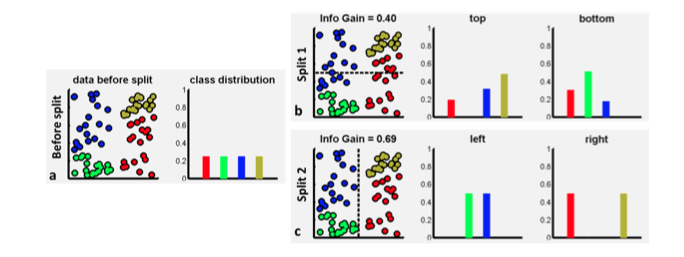
\includegraphics[width=0.8\linewidth]{InformationGain.png}
	\caption[Information Gain for discrete, non-parametric distributions]{\label{fig:IG}}  \textbf{Information Gain for discrete, non-parametric distributions} \cite{DFMS}
\end{figure}

\subsection{Random Forest}
\label{subsec:RF}

\begin{definition}
\label{def:Random forest}
	A random forest an ensemble of randomly trained decision trees with randomized collection of features at each split \cite{DFMS}.
\end{definition}
In general, random forest is distributed algorithm which means that trees are trained in parallel. Trees in a random forest are learned from randomly sampled subsets of data which reduces over-fitting compared to training on the whole data set. \cite{GFRF, MVDT,RFML} The other randomness which is often used during the training stage of the random forest is a random subset of splits for optimizing the information gain at non-leaf nodes\cite{GFRF}. Compared to other methods such as boosting, random forest has the advantage of searching only in a subset and because of the reduced size of the tests set for each tree, faster training time can be obtained and the collection of the trees at testing time is proved to be more accurate in prediction.  And overfitting can be avoided by setting the maximum depth of the tree at the beginning. At testing time, unseen data is pass to all trees in the forest during which binary test at each node of every tree is performed until the leaf node is reached. After the process, the forest will gather all class distributions of the leaves and produce an average value for the estimation as described in \eqref{eq:randomforestclassification}. Where $ \probability{P}(c|\mathbf{v})$ is the average probability of data point \textbf{v} belonging to class \textbf{c} and $\mathbb{P}_{t}(c|\mathbf{v})$ is the probability of data point \textbf{v} belonging to class \textbf{c} in one tree.
\begin{equation}
\label{eq:randomforestclassification}
	\probability{P}(c|\mathbf{v}) = \frac{1}{T}\sum\limits_{t=1}^T \mathbb{P}_{t}(c|\mathbf{v})
\end{equation}
This the most general version of random forest. There are variations regarding to this report such as the goal of the forest where not classification but regression is needed. These variations will be discussed along with the implementations in the later chapters.
